\chapter{Body of my thesis}
\label{chapter:body}
\thispagestyle{myheadings}

% set this to the location of the figures for this chapter. it may
% also want to be ../Figures/3_Body/ or something. make sure that
% it has a trailing directory separator (i.e., '/')!
\graphicspath{{3_Body/Figures/}}

\section{Some results}
\label{sec:results}

Here goes all the important stuff, likely with a lot of graphics like this:

\begin{figure}[htb]
  \begin{minipage}[t]{0.49\linewidth}\centering
    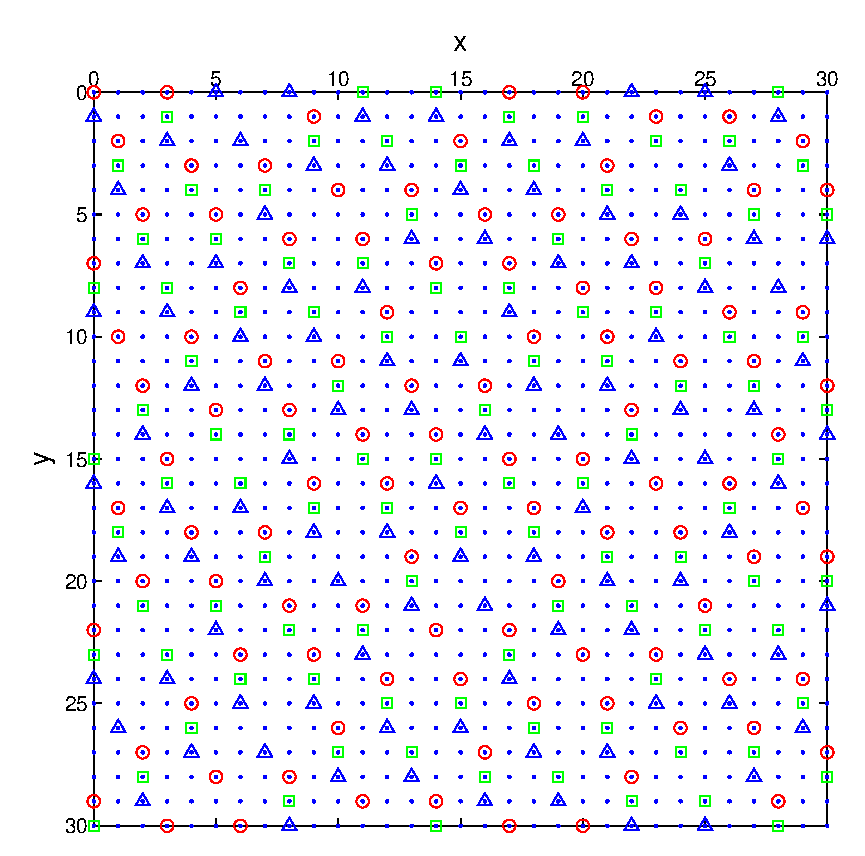
\includegraphics[width=7cm]{figure_sampling_view1.eps}
    \medskip
    \centerline{(a)}
  \end{minipage}\hfill
  \begin{minipage}[t]{0.49\linewidth}\centering
    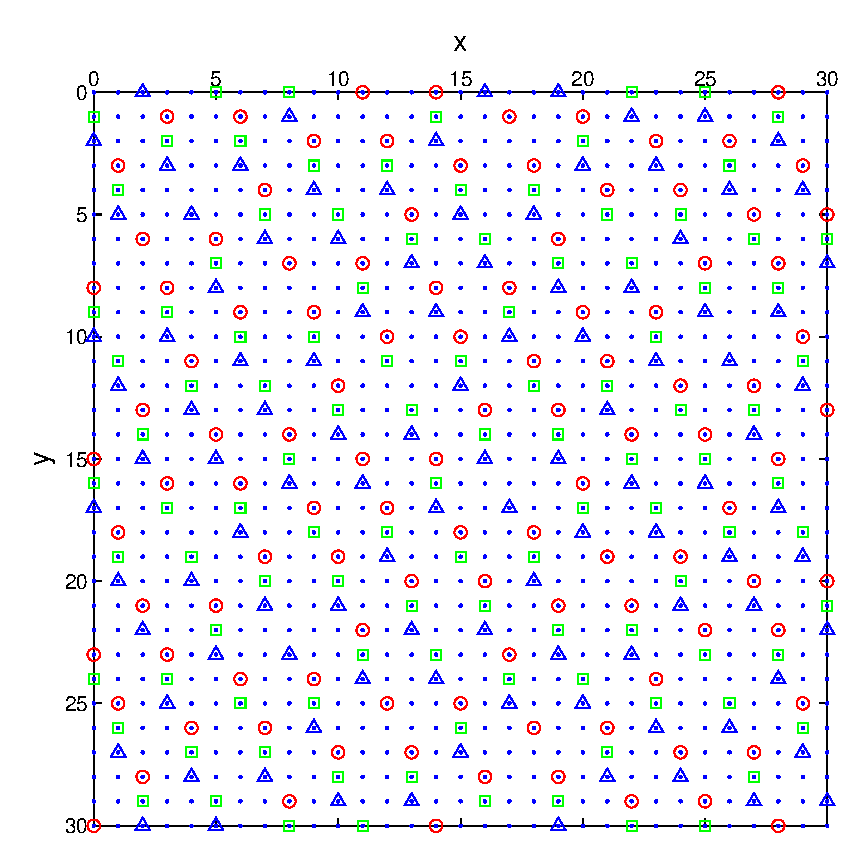
\includegraphics[width=7cm]{figure_sampling_view2.eps}
    \medskip
    \centerline{(b)}
  \end{minipage}
  \caption{Assignment of single-view intensities to RGB components: (a) view
    \#1; and (b) view \#2. }
  \label{fig:Sampling}
\end{figure}

You will also be using a lot of citations. Here is the format required in the dissertation: \cite{lamport1985:latex},\cite{Debr01}.

In all likelihood, you will need to insert tables. See one example on the next page.
\clearpage

\begin{table}[h]
	\caption{Absolute disparity error per pixel for the test data from
		Fig.~\ref{fig:Sampling} and different parameter values. In each experiment one
		parameter is adjusted while other parameters are unchanged.} 
	\centering
	\begin{minipage}[b]{0.30\linewidth}
		\centerline{$\eta=6000$, $\mu=2000$}\smallskip
		\centering
		\begin{tabular}{ccc}
			\hline
			$K$ & $u_1$ & $u_2$\\
			\hline
			3   & 0.52 &0.46\\
			7   & 0.47 &0.43\\
			10  & 0.35 &0.36\\
			12  & 0.37 &0.36\\
			\hline
		\end{tabular}
	\end{minipage}
	%
	\begin{minipage}[b]{0.34\linewidth}
		\centerline{$K=10$, $\mu=2000$}\smallskip
		\centering
		\begin{tabular}{ccc}
			\hline
			$\eta$ & $u_1$ & $u_2$\\
			\hline
			1000&0.54& 0.45\\
			3000&0.43& 0.40\\
			6000&0.35& 0.36\\
			9000&0.37& 0.37\\
			\hline
		\end{tabular}
	\end{minipage}
	%
	\begin{minipage}[b]{0.32\linewidth}
		\centerline{$K=10$, $\eta=6000$}\smallskip
		\centering
		\begin{tabular}{ccc}
			\hline
			$\mu$ & $u_1$ & $u_2$\\
			\hline
			100 &1.00&1.16\\
			1000&0.53&0.47\\
			2000&0.35&0.36\\
			3000&0.44&0.43\\
			\hline
		\end{tabular}
	\end{minipage}
	%
	\label{tab:Parameters}
\end{table}

\section{Experiment of Memory Allocation}
\label{sec:history}
This experiment is to test how static and dynamic memory allocation of Java and Rust behave. For the assessment, Element addition to ArrayList in the case of Java and Vector in the case of Rust 
is emploied here. These data stractures are resizable and we have control to set initial size. There are two parameters; initial size of ArrayList or Vector and thier final size after additions of elements. 
We are interested in the impact to memory allocation by initial allocation and expantion to runtime.

First, an ArrayList and an Vector are created with specified initial size. Then, in a loop, a element is added for each iteration until the size of the ArrayList or Vector get the specified final size. 
Each data structure has a different resizing strategy. When an ArrayList hits current limit of its size and expands the limit, it doubles the current size.  
While Vector does not have specific strategy for its resizing, the expantions of size of both ArrayList and Vector might affect the digradation of runtime performance.

To perform benchmarks, we use Java Microbenchamrk Hardness (JMH) for Java and Criterion for Rust. The benchmark time is calculated mean from several iterarions. 
We warm up before the execution. The parameters are set in combination of initial size, 10, 100, 1000, and 10000 and final size, 9, 99, 999, 9999. 
The results are shown in Figure 2-4 and 2-5. 

Discussions here are separated to two cases: when initial size is set bigger than final size and when final size is set bigger than initial size. 
For ArrayList in Java, it shows performance significant degradation when the initial size is bigger than final size. When we create ArrayList with intial size of 1000 and add 99 elements 
to the ArrayList, the the average execution time is 1125 ns. However, the average excution time when we create ArrayList with intial size of 100 and add 99 elements is 623 ns. 
This degration is caused by the cost of initializing the large array. On the other hand, Rust Vector does not have significant cost for the initialization of size compared to the cost of addition of elements. 
In the case of Vector with initial size of 1000 and add 99 elements to the Vector, the average excution is 320 ns. In the case of the initial size of 100 and 99 elements additions, 
the average excution is 279 ns. This is such small degradation compared to element addition in Vector. 

In ArrayList when the initial size is smaller than the final size, there can be degradation in performance. When its initial size and final size are set 100 and 999 respectively, 
the average execution time is 10884 ns. However when its initial size and final size are set 1000 and 999 respectively, the average execution time is 4250 ns. 
This result shows the degradation of in performance caused by the copy of existing elements into newly allocated array whose size is double of the last array.

This characteristic can be seen in the case of Vector in Rust. Vector with initial size 100 and final size 999 performs the average excution time 3514 ns, 
but one with initial size 1000 and final size 999 performs 2723 ns. When the Vector reachs its capacity, it allocates a larger buffer and copies the present elements to it.
This cost results in the degradation of the average excution time.

\begin{figure}[htb]
    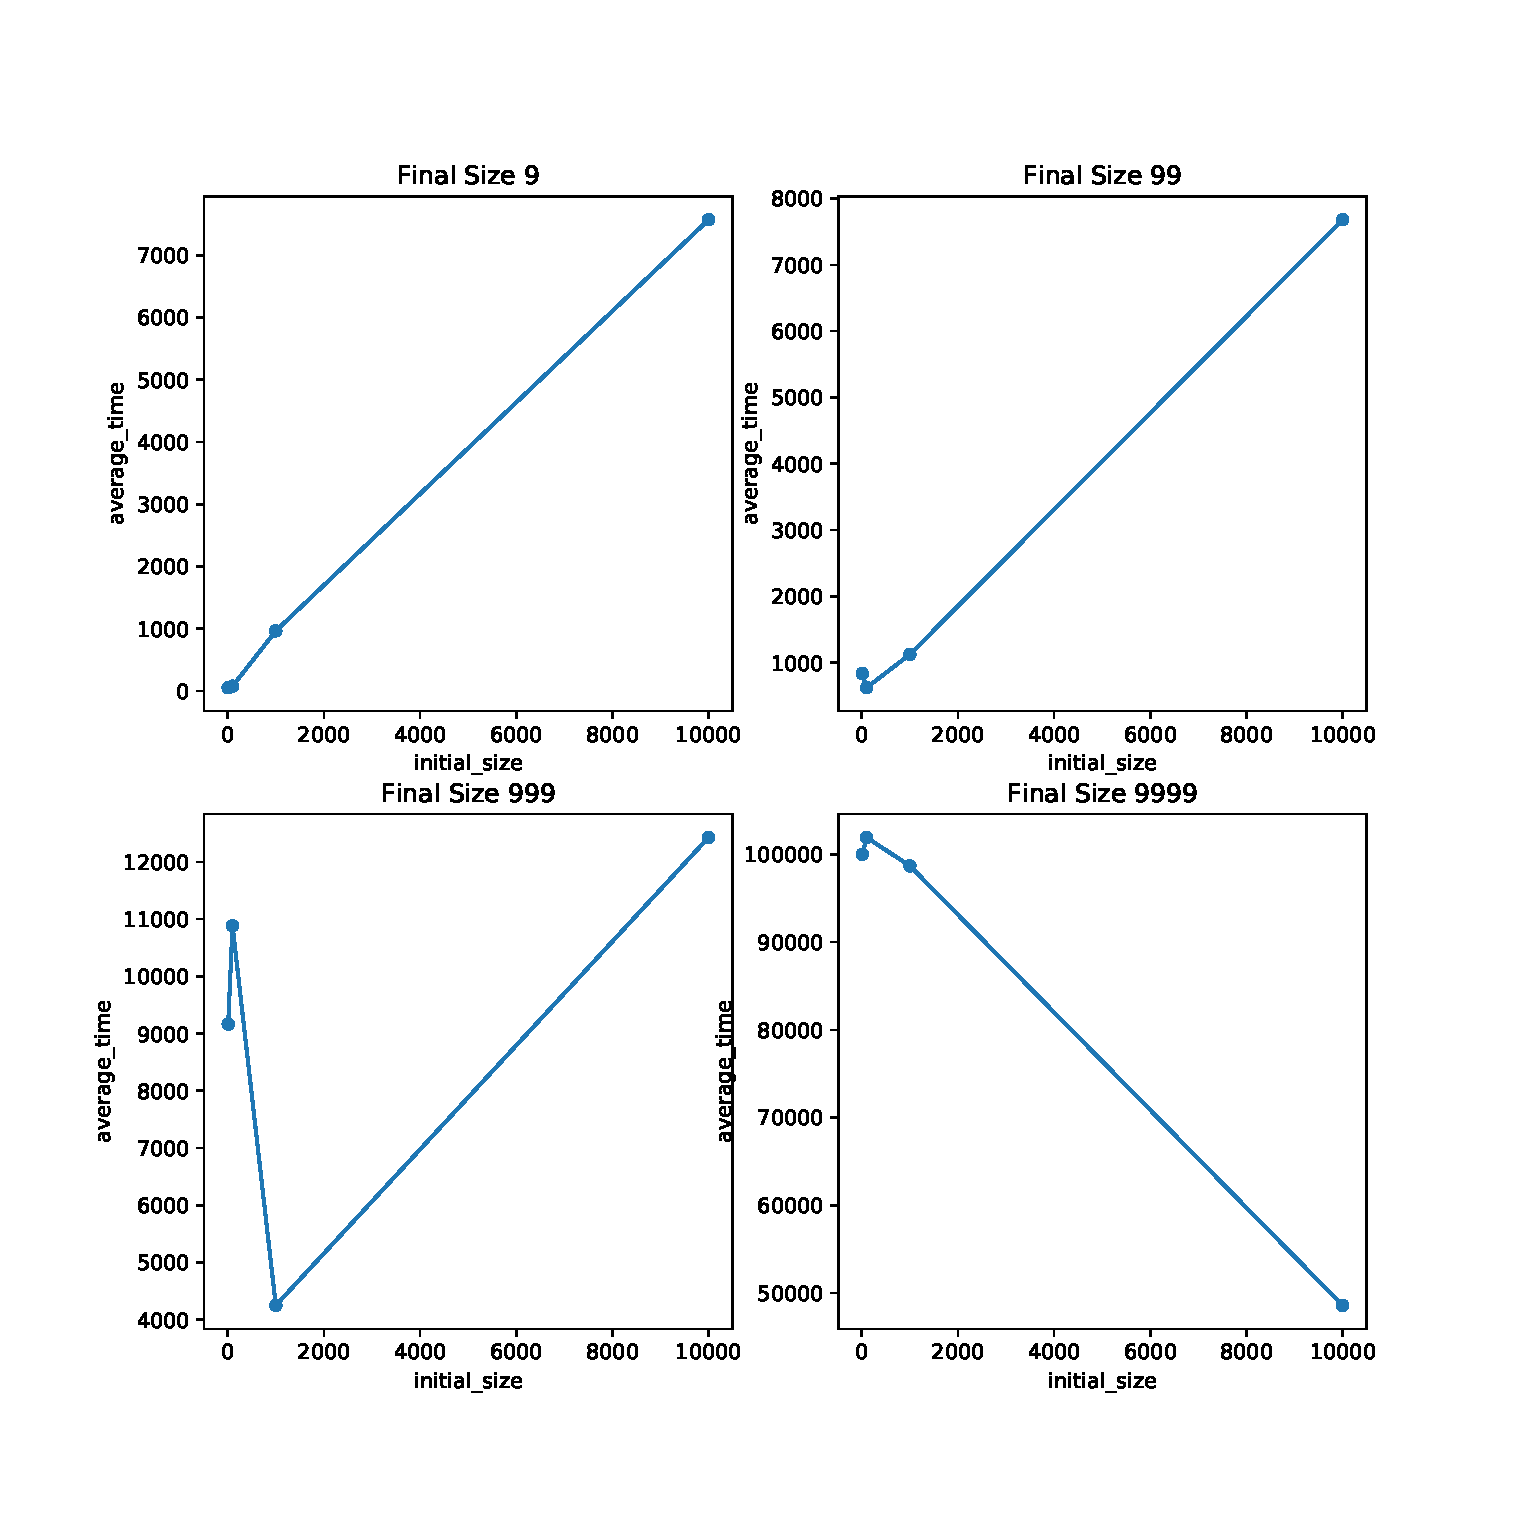
\includegraphics[width=15cm]{java_arraylist.eps}
    \caption{Memory allocation of ArrayList in Java}
    \label{fig:Sampling}
\end{figure}

\begin{figure}[htb]
    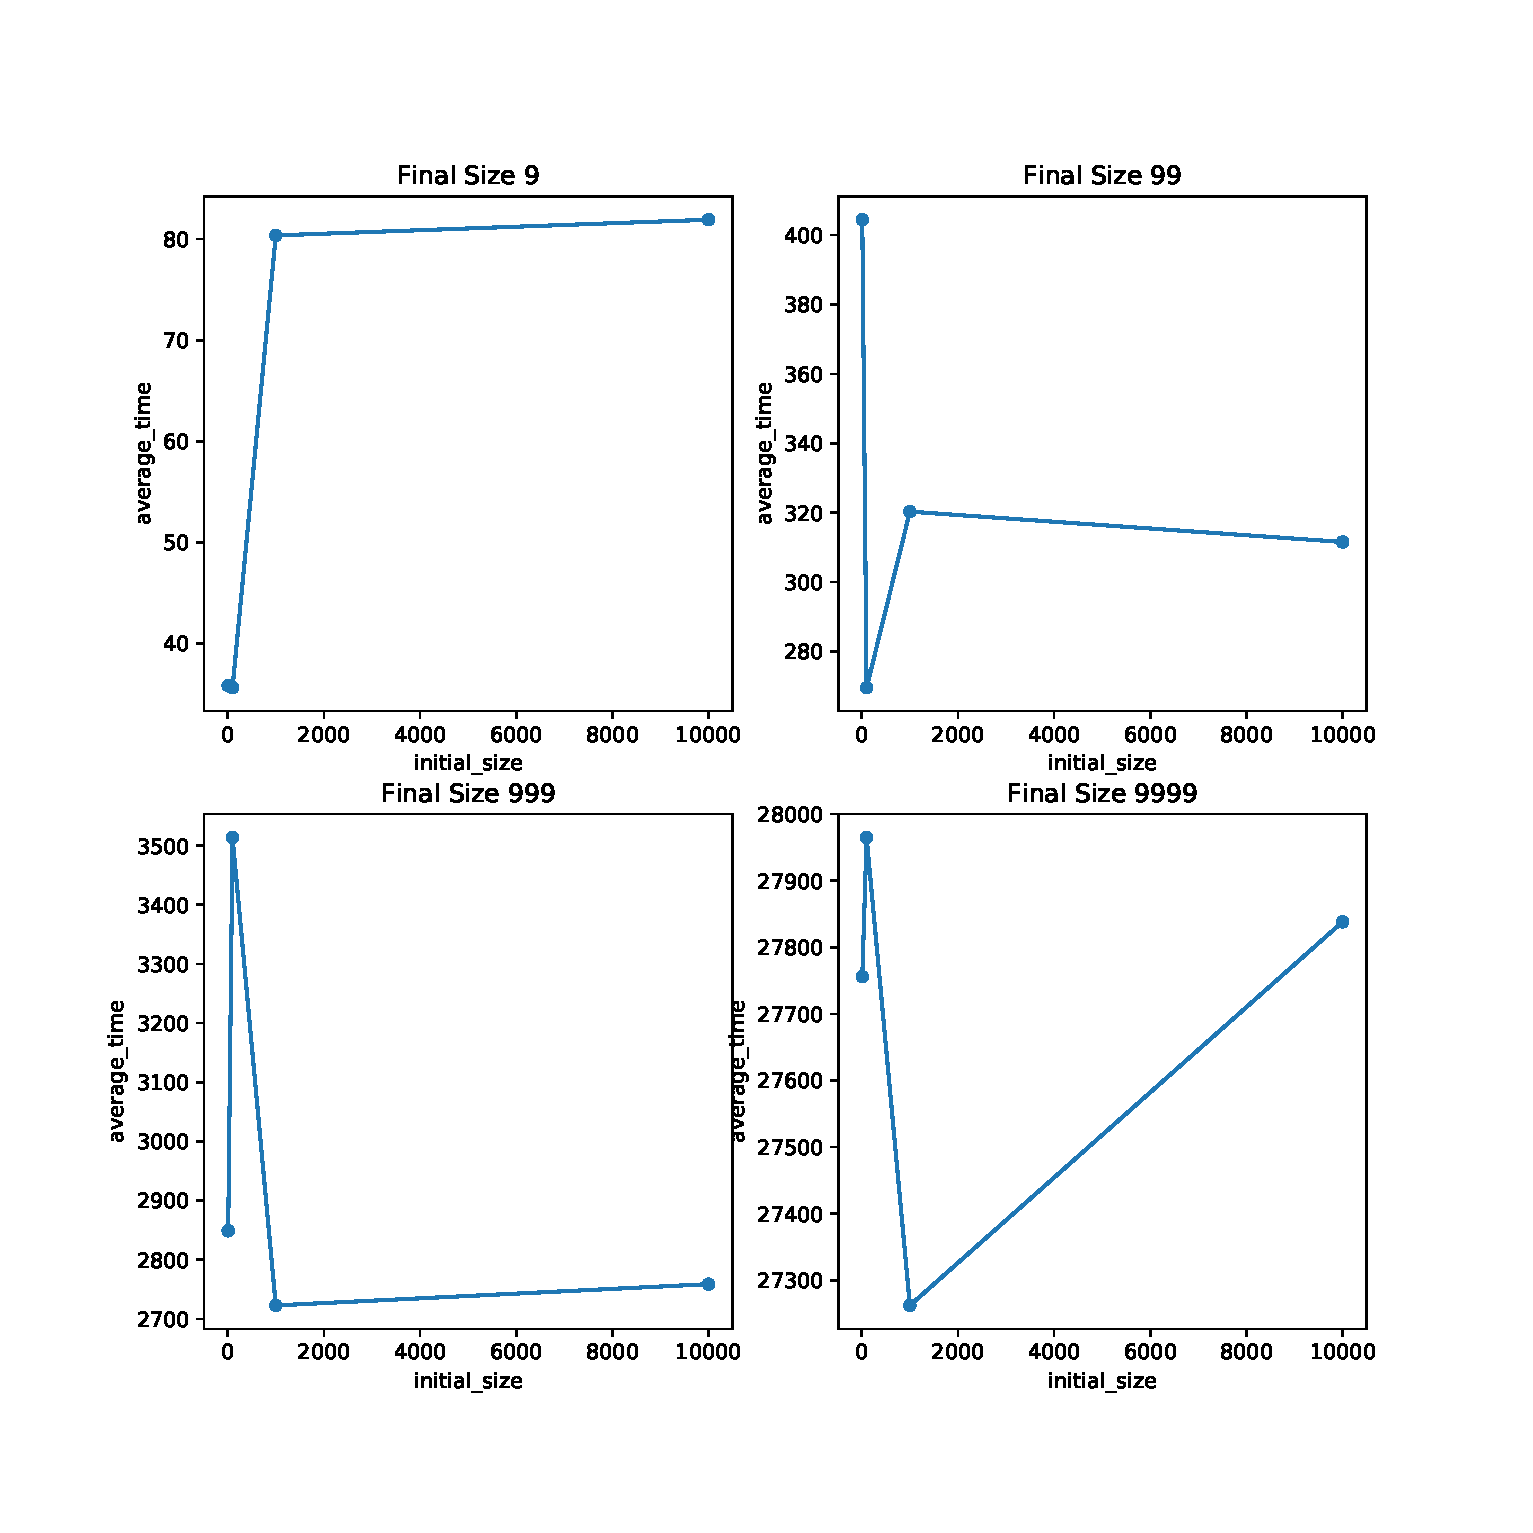
\includegraphics[width=15cm]{rust_vector.eps}
    \caption{Memory allocation of Vector in Rust}
    \label{fig:Sampling}
\end{figure}




\section{Experiment of Memory Allocation for Different Element Type.}
\label{sec:history}
This experiment is to test how static and dynamic memory allocation of Java and Rust behave. For the assessment, Element addition to ArrayList in the case of Java and Vector in the case of Rust 
is emploied here. These data stractures are resizable and we have control to set initial size. There are two parameters; initial size of ArrayList or Vector and thier final size after additions of elements. 
We are interested in the impact to runtime performance by initializing memory allocation and dynamicaly allocating memory space.

First, an ArrayList and an Vector are created with specified initial size. Then, in a loop, a element is added for each iteration until the size of the ArrayList or Vector get the specified final size. 
Each data structure has a different resizing strategy. When an ArrayList hits current limit of its size and expands the limit, it doubles the current size.  
While Vector does not have specific strategy for its resizing, the expantions of size of both ArrayList and Vector might affect the digradation of runtime performance.

Second, four types of element are used for elements addition to each data structure: integer, array of charactors, string, and Customer object. 
Assamption is that there would be different behavior between element additions of dynamically resizable and static size objects. 
Customer object has three fields. These fields are total order, weight of order, and zip code whose types are integer (i32 in rust), double (f32 in rust), and string respectively.
Figure 2-6 and 2-7 are representations of customer objects in Java and Rust.

Figure 2-10, 2-11, 2-12, and 2-13 represent the result of the experiments. For both data structures, integer elements addition shows the fastest runtime among all object types. 
This is because the compilers know each integer need 4 bytes to be stored in memory so that the space for memory that should be allocated is easily inspected. 
For the same reason, the initialization of data structures whose elements are integers alaways improves runtim performance.

The elements addition of strings and array of character behave similally among each languages. These two types of elements addition perform the similar speed and significantly slower than integer addition. 
Customer object addition is the slowest in Java. However, in Rust the addition of Customer object is the second fastest among all element typs.
The impacts of initialization of Java ArrayList vary among elemet types. On the other hand, the initailization Rust Vector always improves runtime performance for any of 4 types of elements addition.


\begin{figure}[htb]
    \begin{lstlisting}
        class Customer {
            int totalOrder;
            double weightOrder;
            String zipCode;
        }
    \end{lstlisting}
    \caption{Representation of Customer object in Java.}
    \label{fig:Sampling}    
\end{figure}

\begin{figure}[htb]
    \begin{lstlisting}
        struct Customer {
            total_order: i32,
            weight_order: f32,
            zip_code: String,
        }
    \end{lstlisting}
    \caption{Representation of Customer object in Rust.}
    \label{fig:Sampling}
\end{figure}

\begin{figure}[htb]
    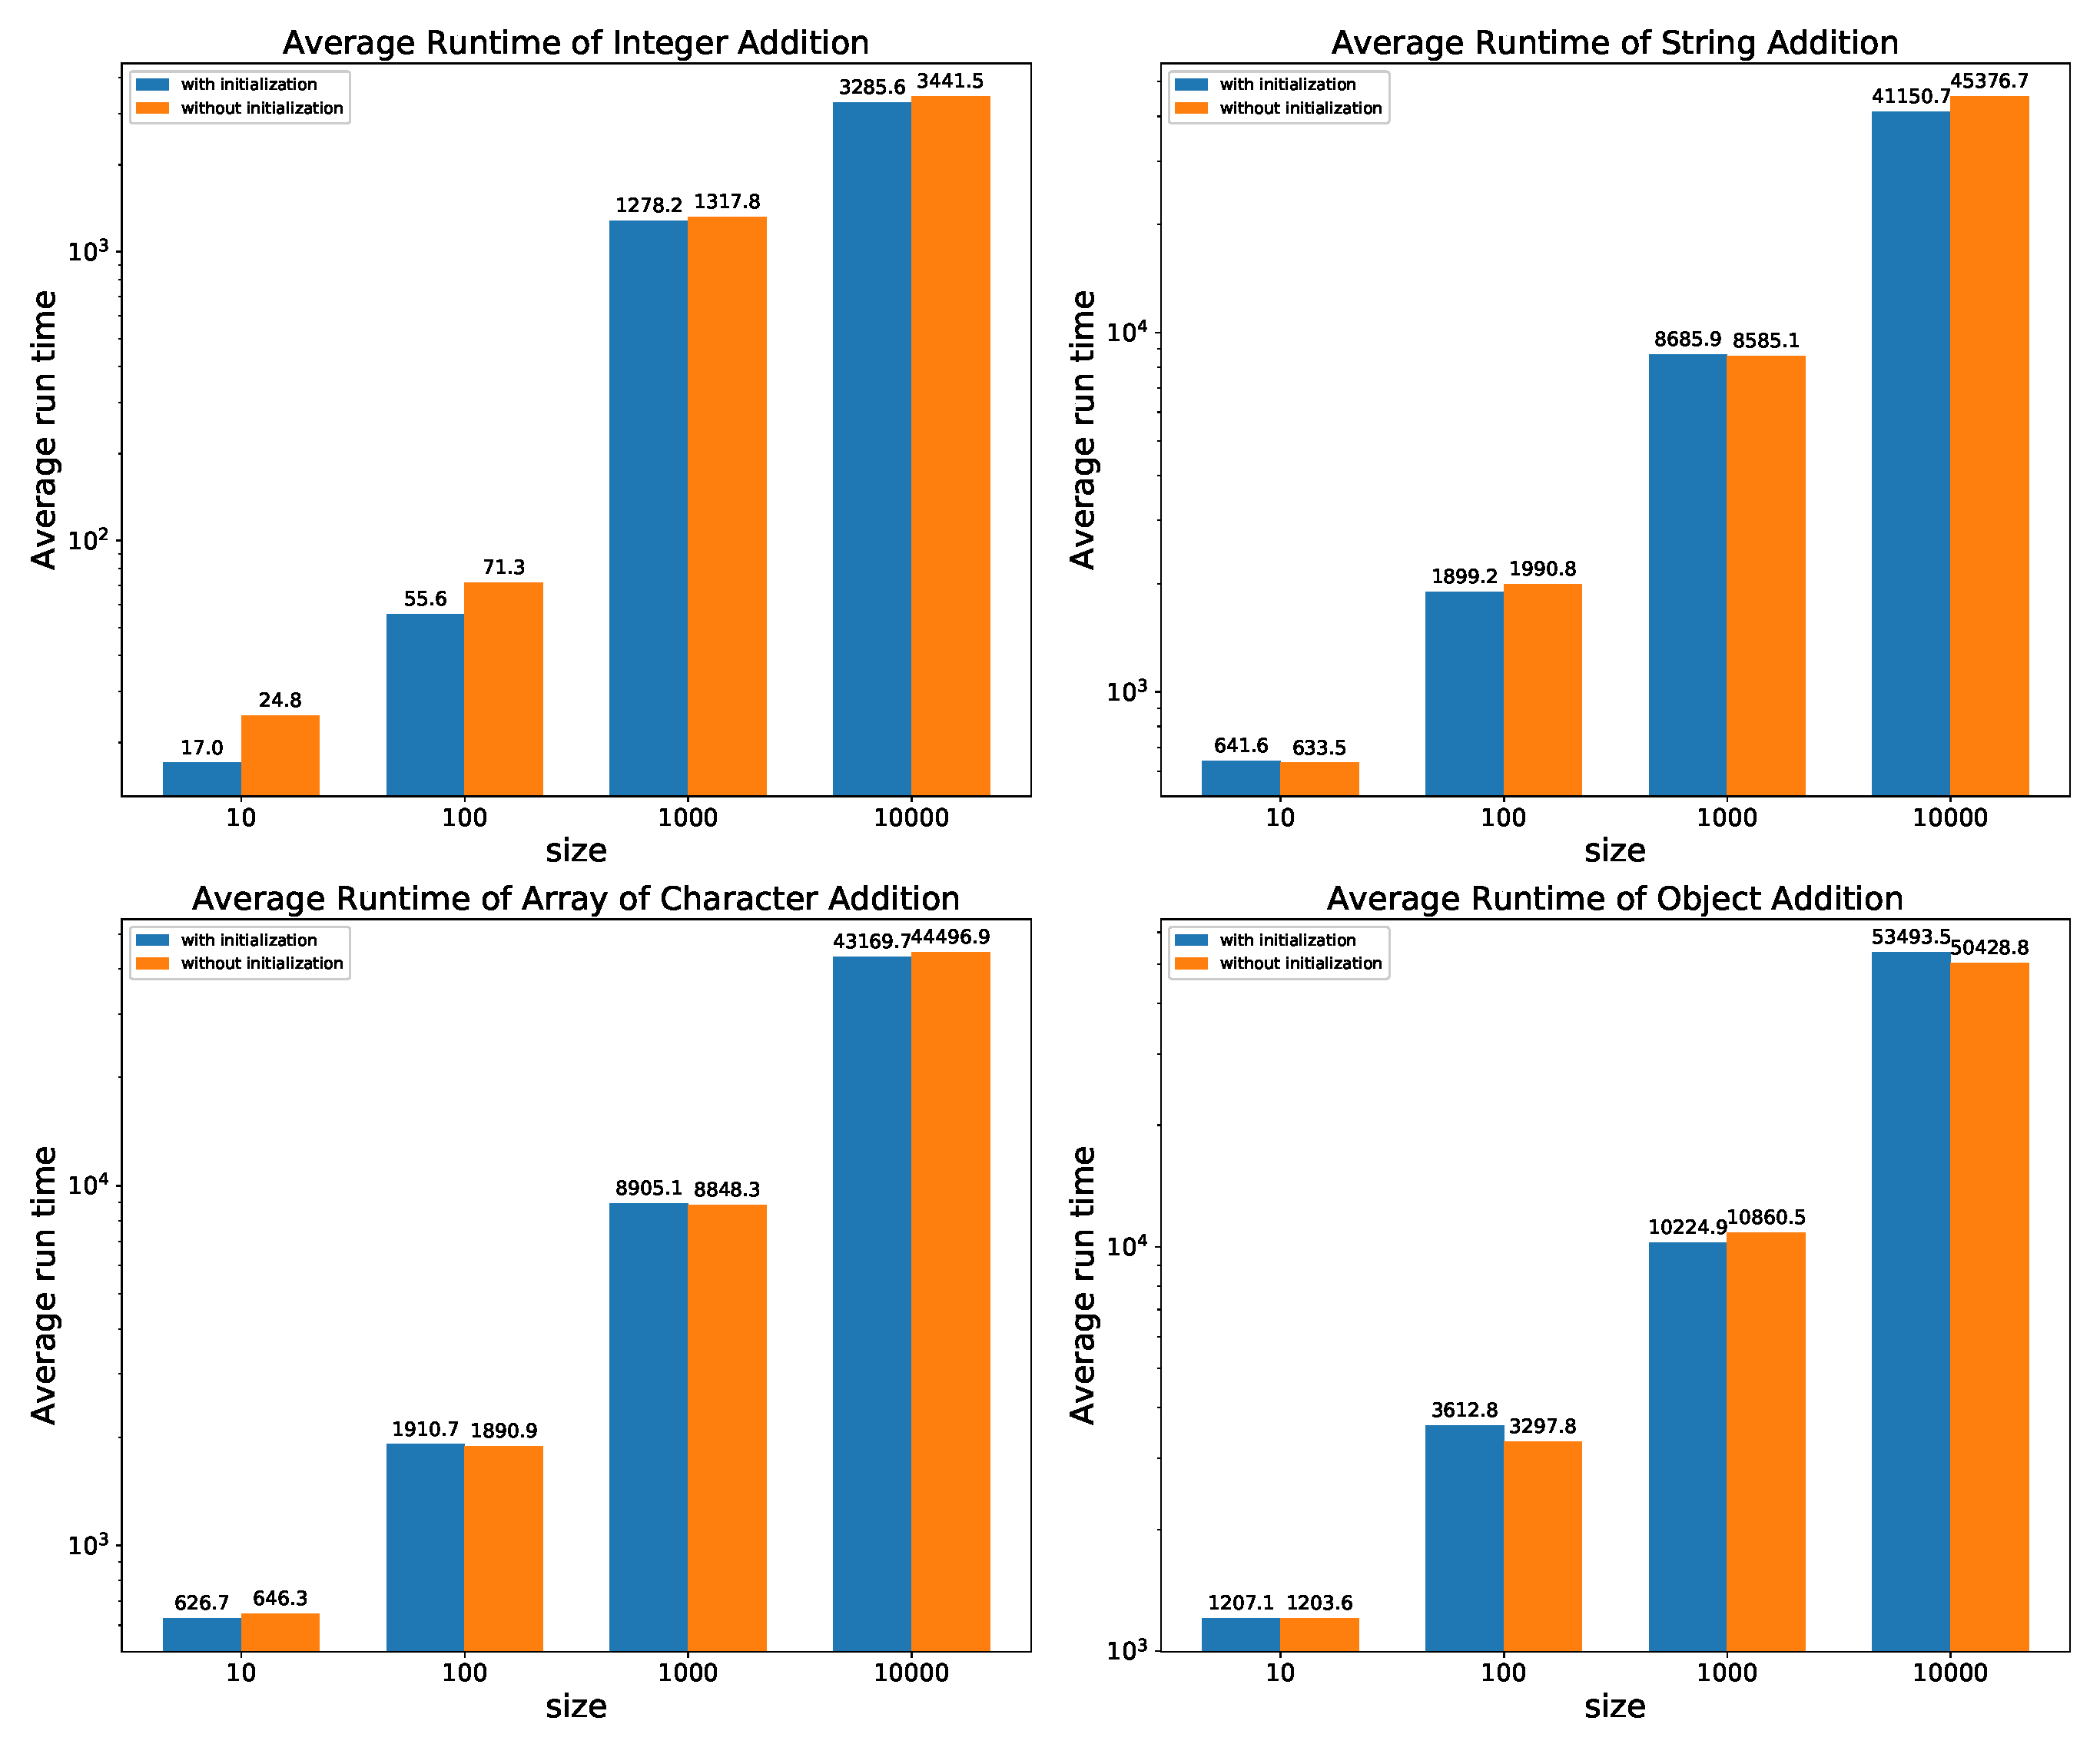
\includegraphics[width=15cm]{java_arraylist_log.eps}
    \caption{Memory allocation of Java ArrayList}
    \label{fig:Sampling}
\end{figure}

\begin{figure}[htb]
    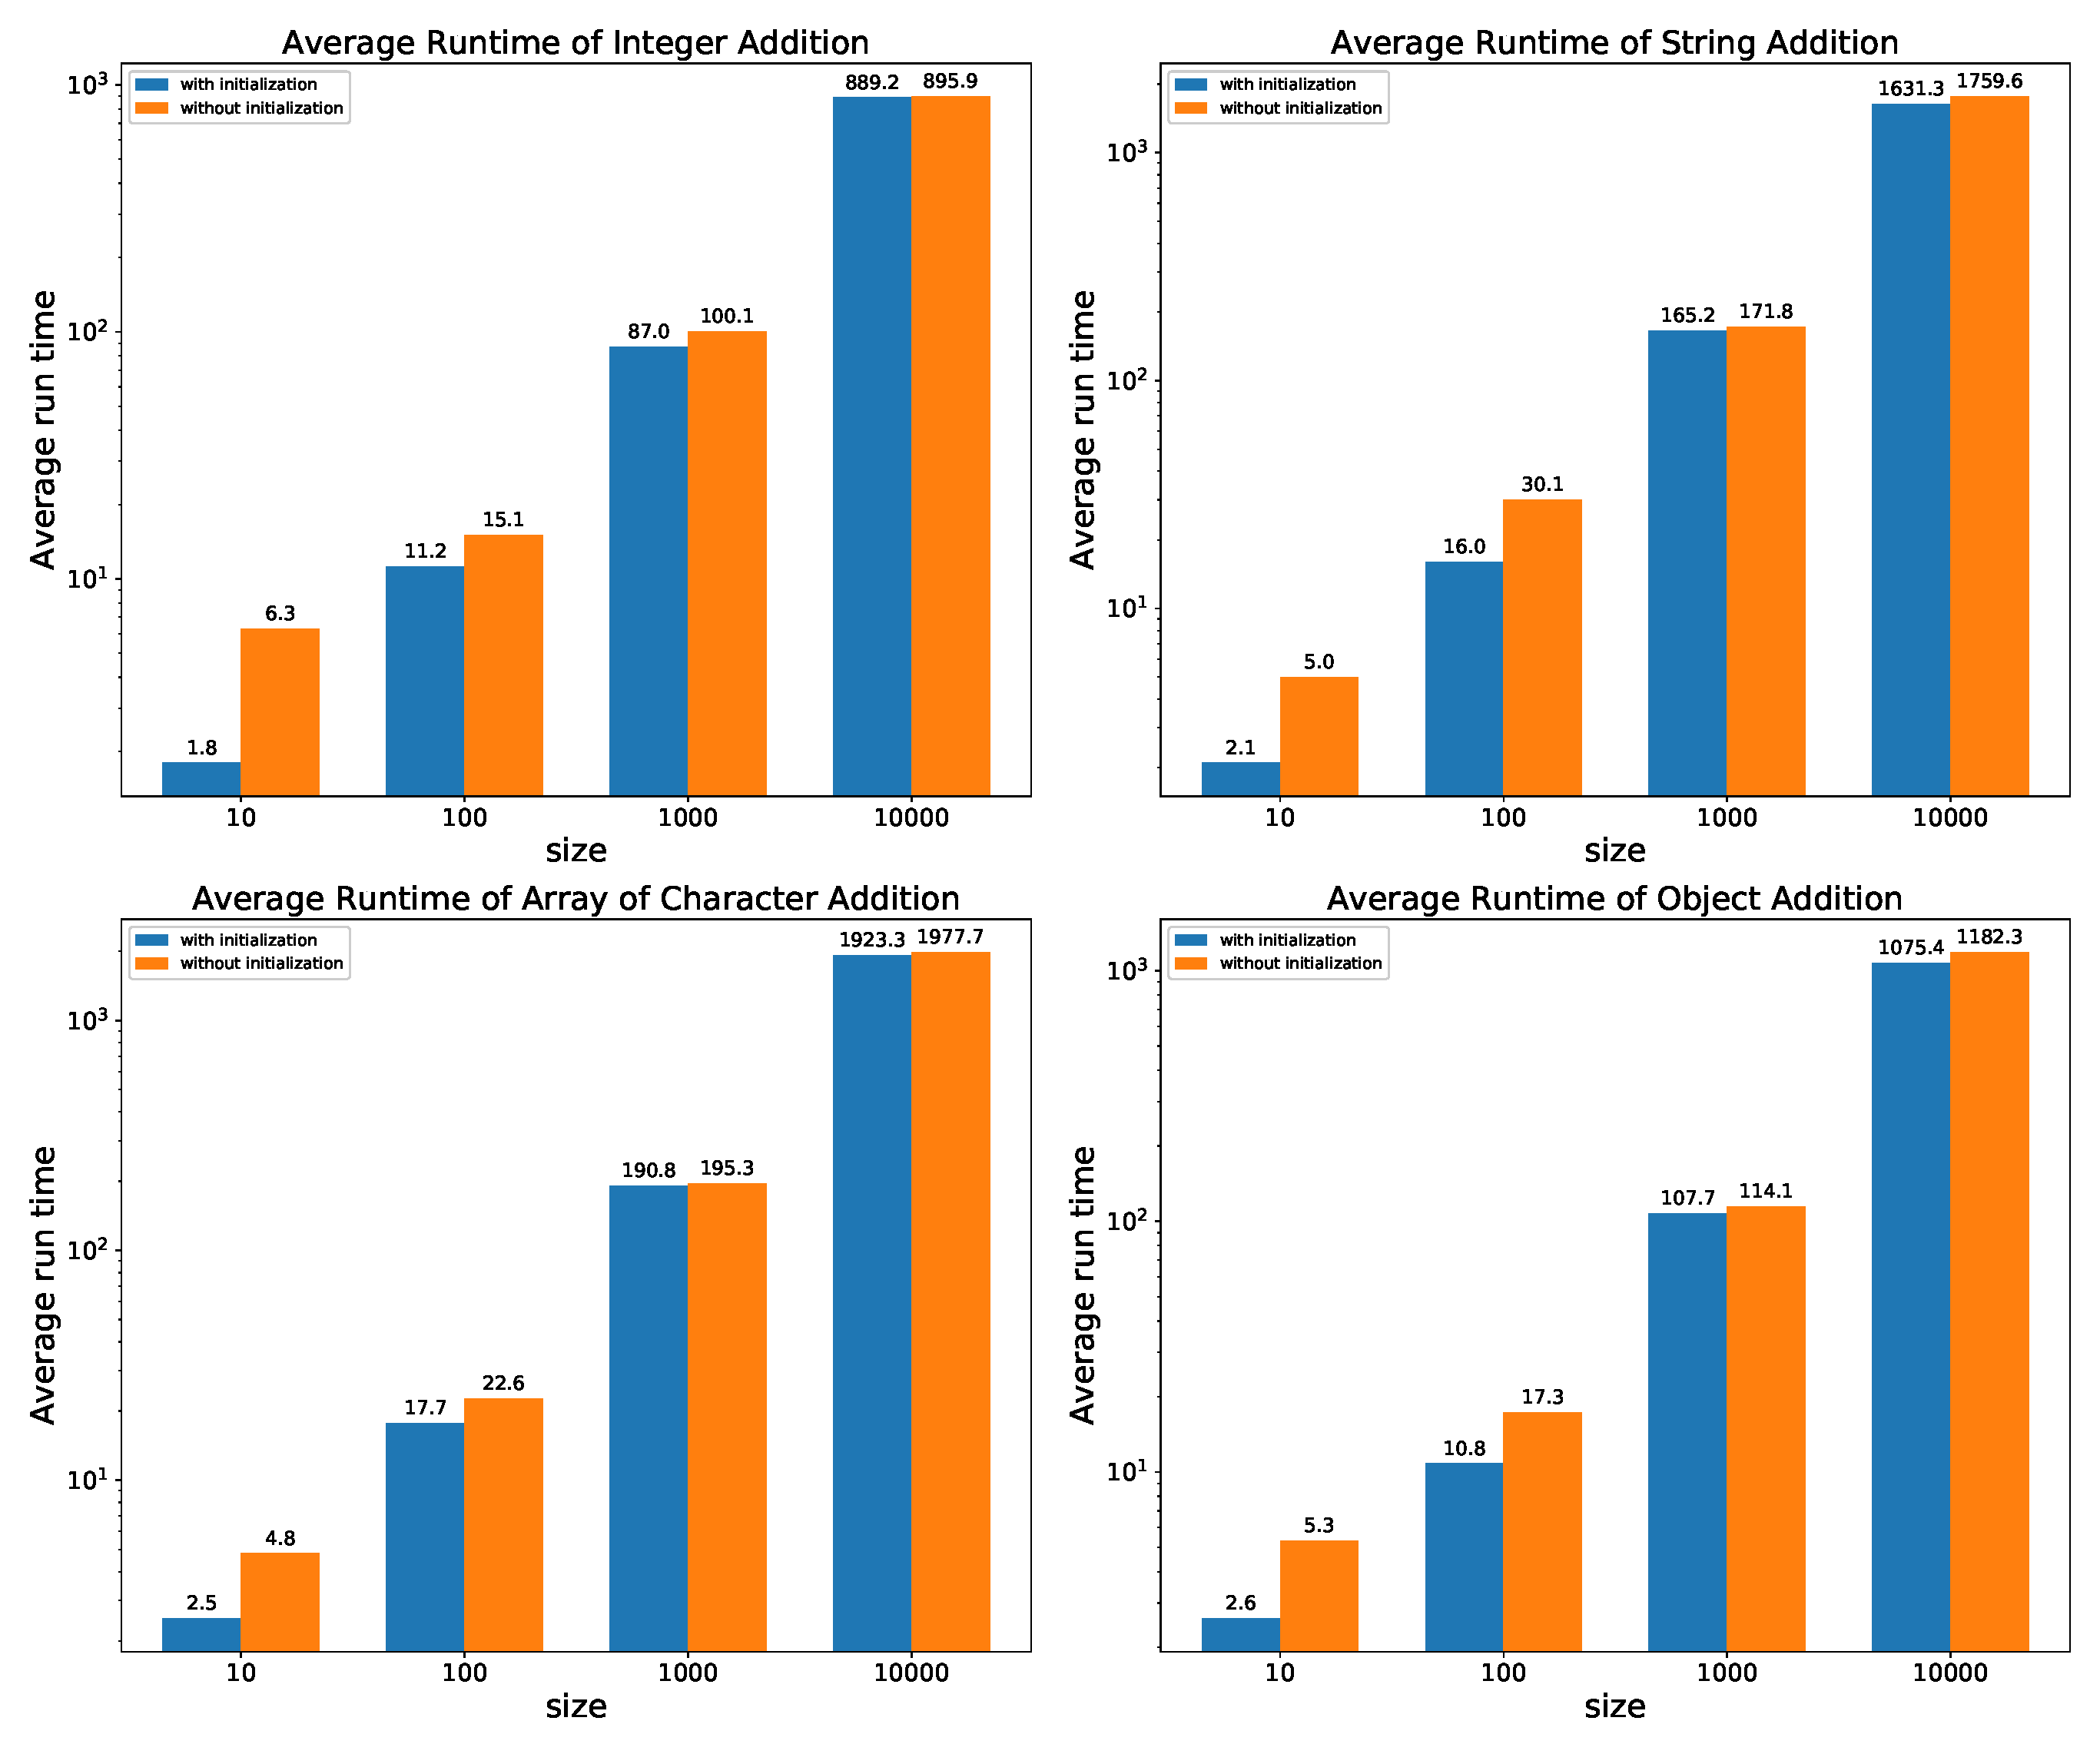
\includegraphics[width=15cm]{rust_vector_log.eps}
    \caption{Memory allocation of Rust Vector}
    \label{fig:Sampling}
\end{figure}


\begin{figure}[htb]
    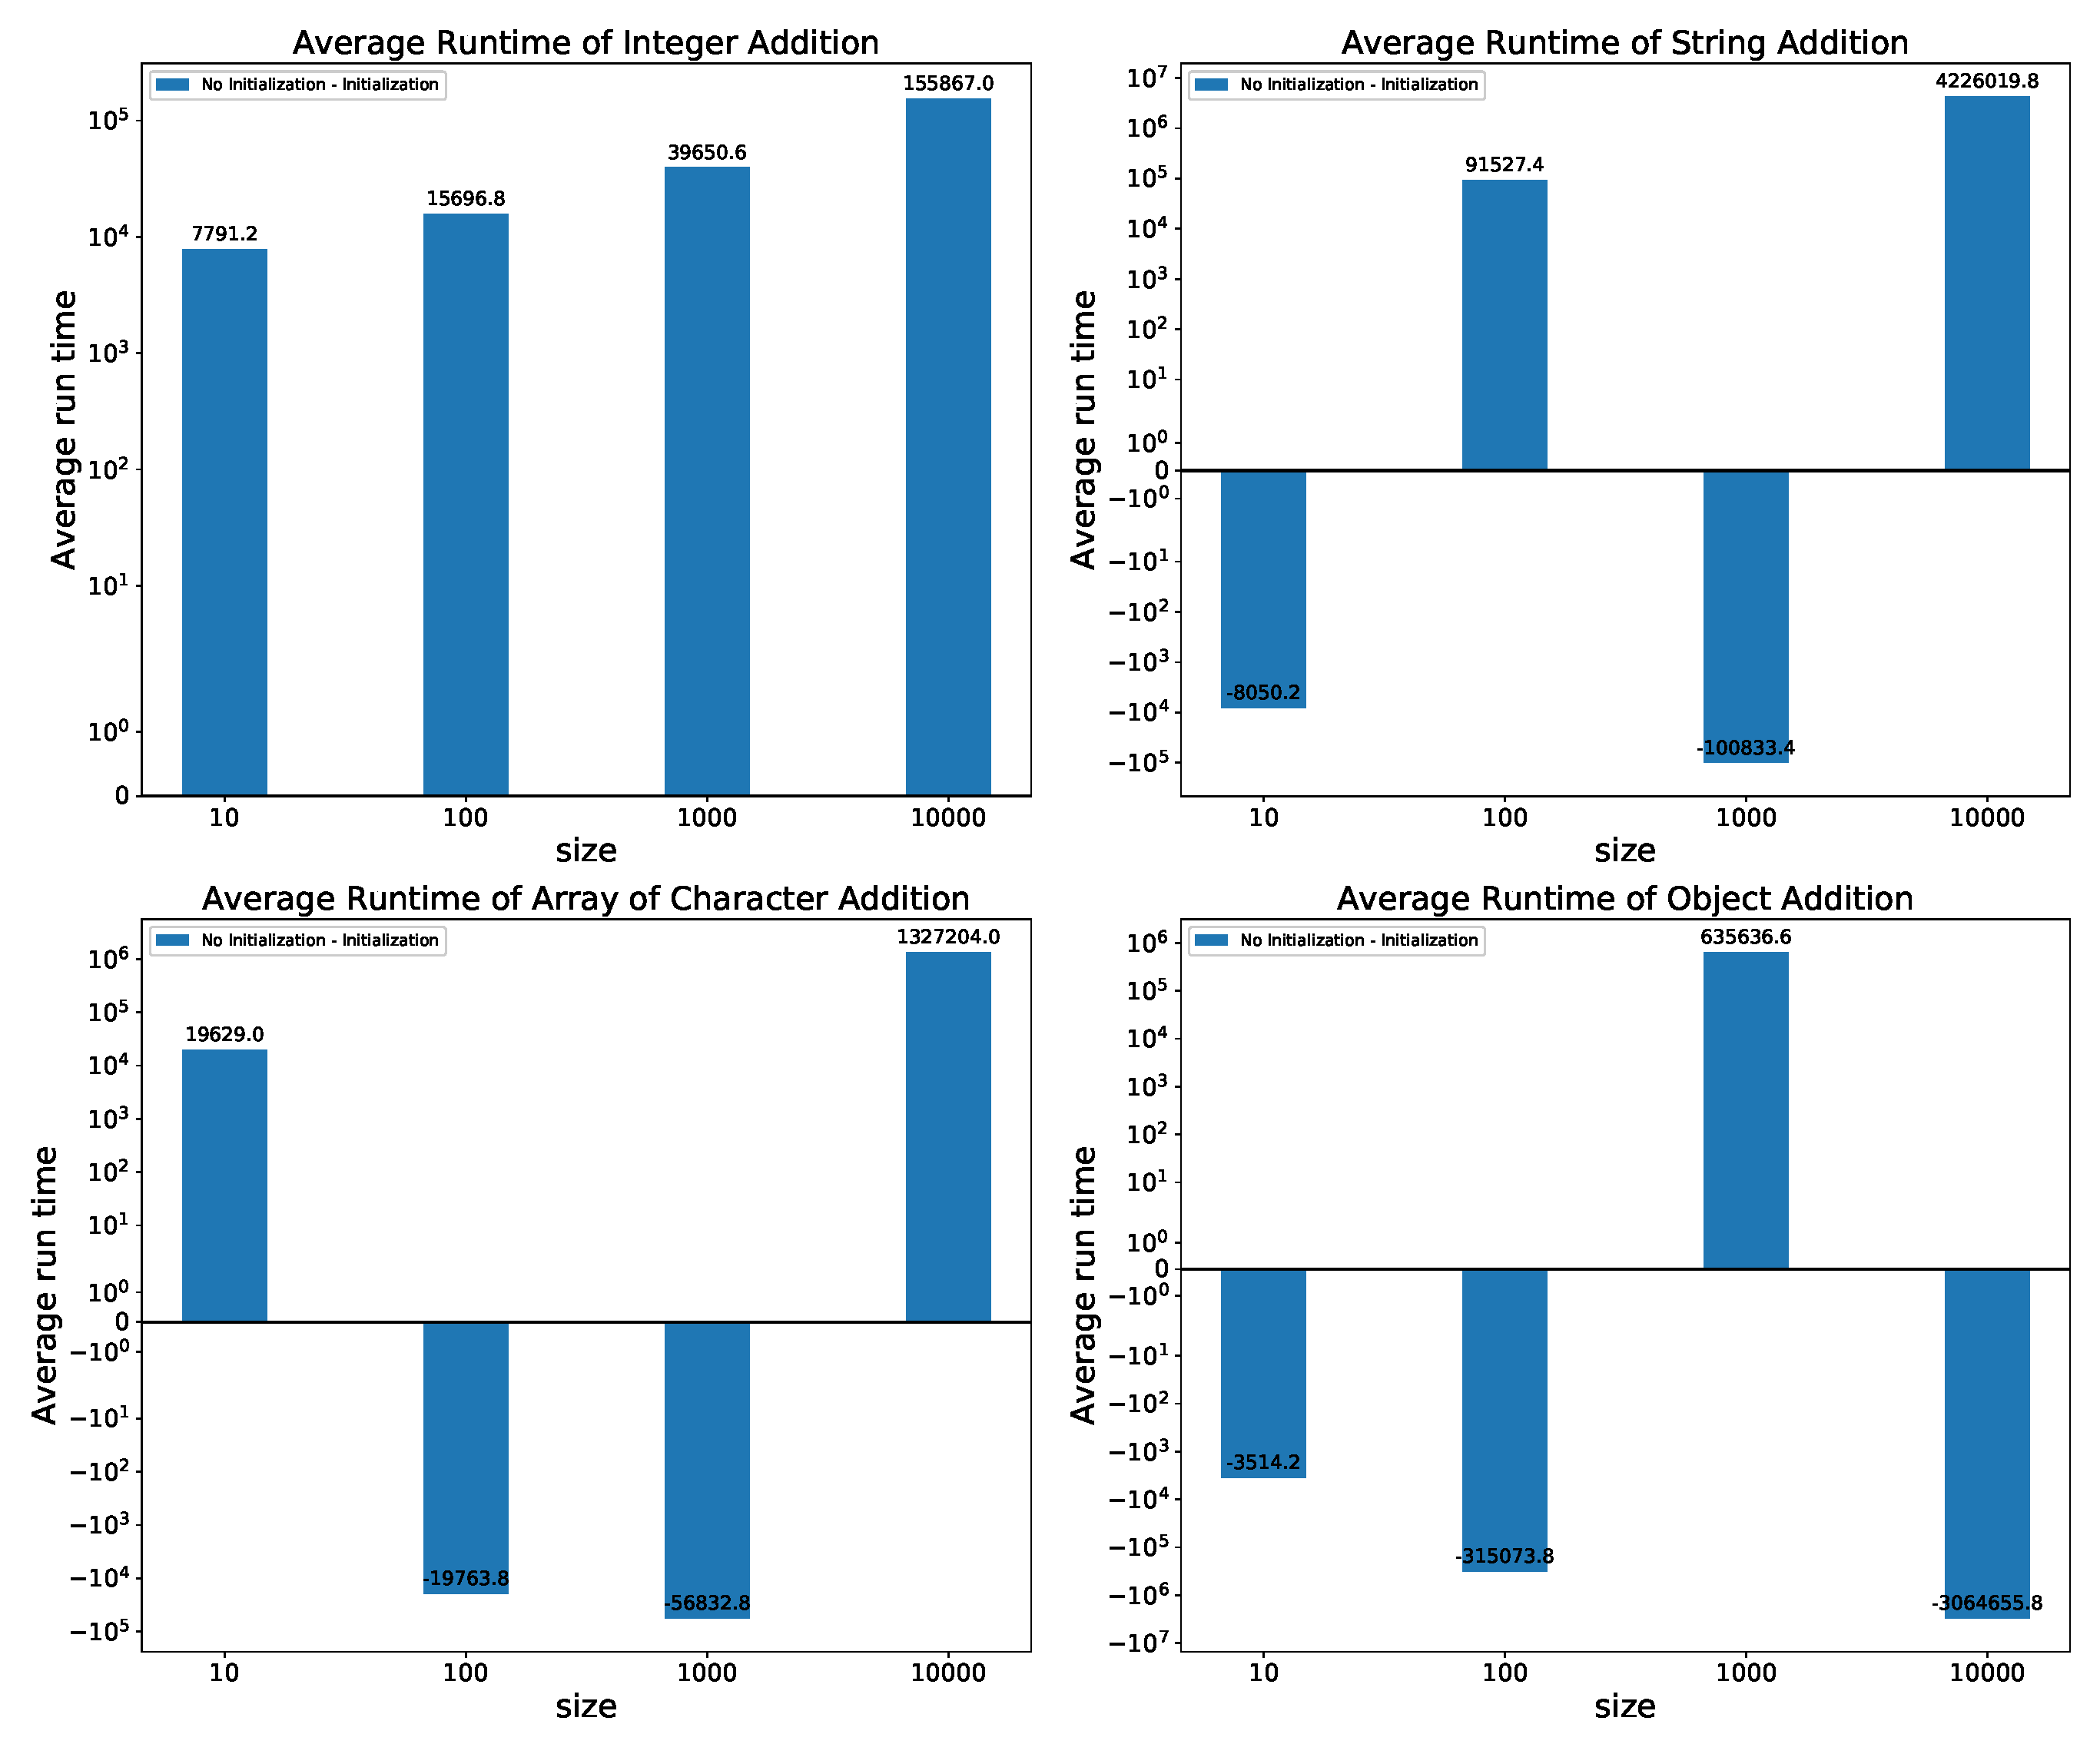
\includegraphics[width=15cm]{java_arraylist_difference.eps}
    \caption{Difference of Memory allocation of Java ArrayList between Non-initialization and Initialization}
    \label{fig:Sampling}
\end{figure}

\begin{figure}[htb]
    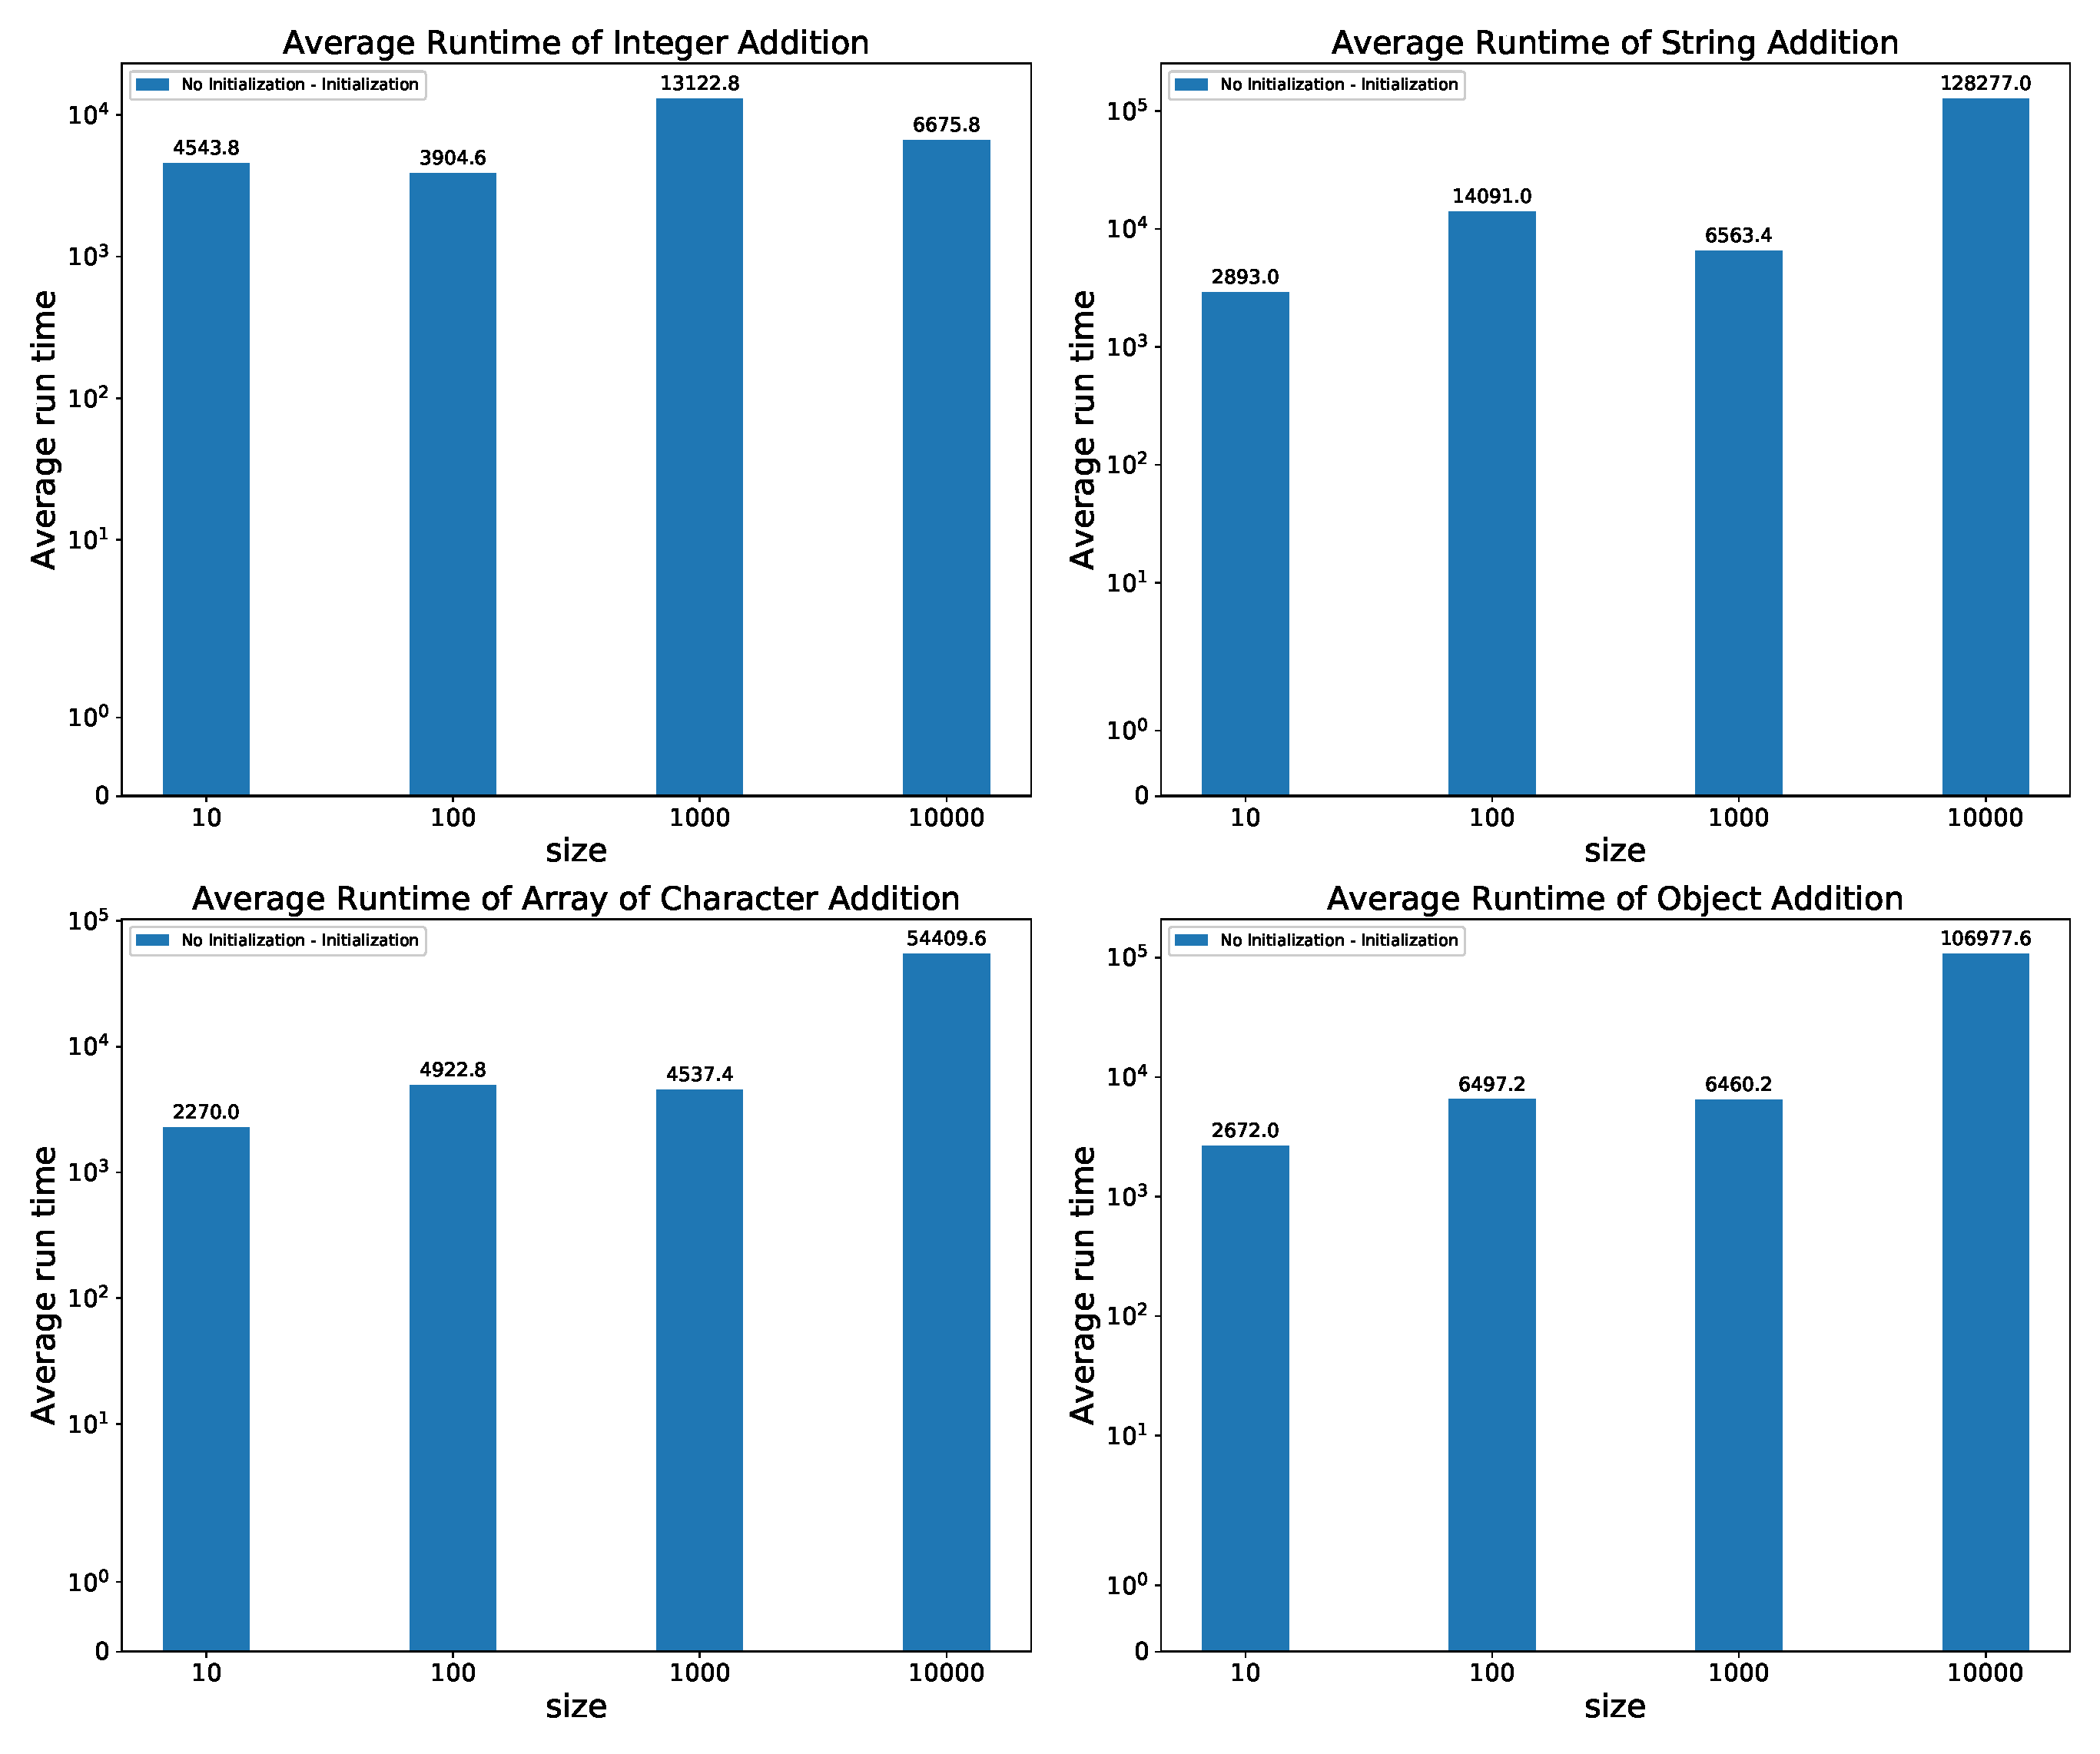
\includegraphics[width=15cm]{rust_arraylist_difference.eps}
    \caption{Difference of Memory allocation of Rust Vector between Non-initialization and Initialization}
    \label{fig:Sampling}
\end{figure}

\section{Experiment for Tree-aggregation}
\label{sec:history}
\subsection{Description}
Tree-aggregate is a communication patten heavily used for Machine Learning algorithm in Spark (MLlib). 
In the traditional aggregation function in Spark, results of aggregation in all executor clusters are sent to the driver. 
That is why this operation suffers from the CPU cost in merging partial results and the network bandwidth limit.
Tree-aggregate is a communication pattern which overcomes these problems by breaking aggregate operation in multi-level represented like tree structure.

In our experiment, tree-aggregation algorithms are examined in multi-threading. This experiment is to evaluate the impact of having Arc (Atomic Reference Counting) as elements of vector. 
In Big Data mining tool, such as Spark, it generates intermediate objects from original source vector. In tree-aggregation, aggregated HashMap like data structure is created in each step or node. 
Acquisition of elements in source vector is required to perform this aggregation. There are several ways.

One way is deep-copy elements of vector. This solution allocated newly created objects by deep-copy. 
Aggregation is performed on copied objects, stores them in the data structure and sends it to next node. 
Deep-copy generates duplicates of objects in vector and aggregated data structure. 
This can lead to memory intensive moment when we need memory space for the duplicated objects in addition.

The other way is to get reference to the elements. Since an original source vector is deallocated after a local aggregation,
Simple reference to elements does not live long enough and allow the aggregation result to be sent to next node. 
Instead of simple borrowing, we need owner in the aggregation result. Reference Counting (Rc) in Rust is a way to have multiple owners to a value. 
Since our experiment is implemented in multithreading, Atomic Reference Counting (Arc) is used instead of Rc. With Arc, multiple ownership pointer can be 
possessed by different variables across multiple threads. Therefore a value is not deallocated until all of owners to it are dropped. 
This does not require extra memory allocation, because only acquisition of new ownership to value is needed. 
However, deletion of Arc type checks whether the value is still owned by other variables. 
This checking may be a overhead in algorithms where generate a lot of intermediate data structures, because deletion of the data structures occurs in frequent.

Two algorithms are implemented using the above two different methods and evaluated their runtime performance. 
The both algorithms perform tree-aggregation where runs seven nodes. 
Each node load Customer vector from disk and aggregate it by Customer last name. Once a node finishes aggregation, it sends result to parent node. 
After parent nodes receive aggregation results from all of its children nodes, it joins all aggregation results including its and sends next parent. 
One algorithm performs aggregation by deep-copying elements from source vector loaded from disk. In the other algorithm, each element of source vector 
is wrapped in Arc, and its reference is acquired while aggregation. 


\subsection{Result}

Figure shows runtime performance of two tree-aggregate algorithms. The runtime of algorithm with deep-copy is slower than algorithm with Arc for every vector size. 
This is result of overhead of deep-copy is larger than deletion of Arc. 

\begin{figure}[htb]
    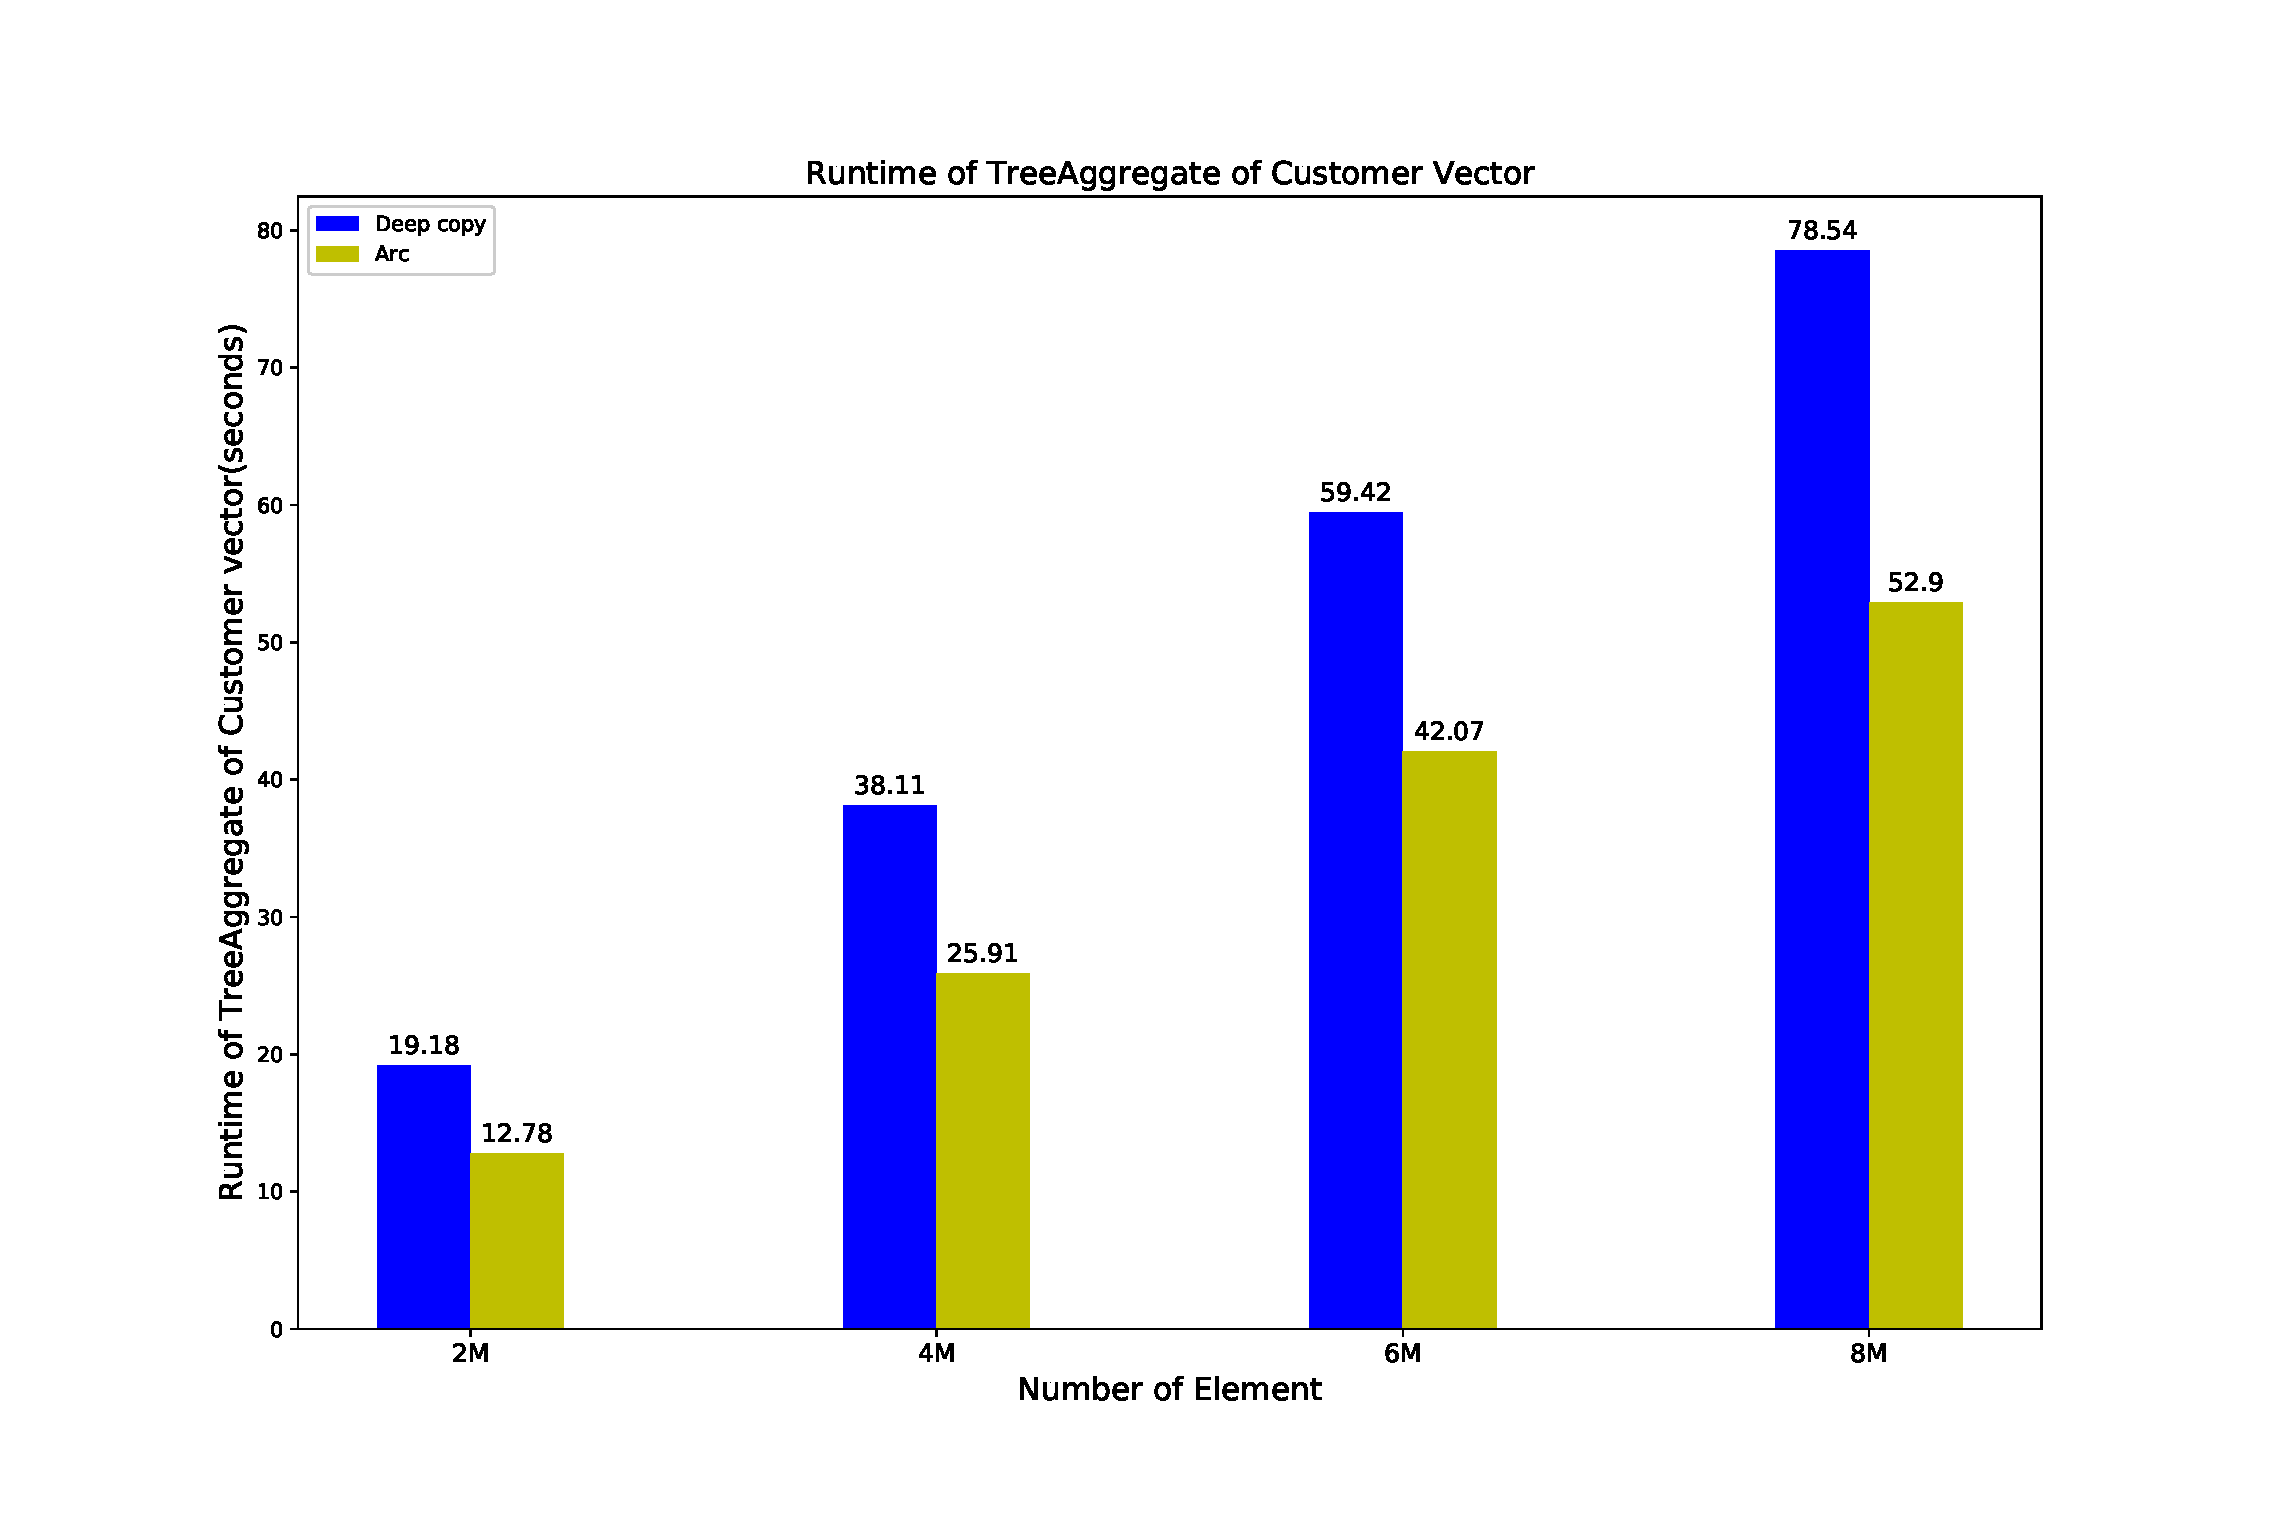
\includegraphics[width=15cm]{rust_tree_aggregate.eps}
    \caption{Runtime of Tree-aggregate algorithm}
    \label{fig:Sampling}
\end{figure}

\subsection{Discussion}
As we explained, Arc has overhead to be deleted because it has to check if the value is still referred. 
Even though the deletion of Arc is slow, deep copy of complex objects has more impact in deterioration of runtime performance. 
In the algorithm with deep copy, the elements of each partition in each node are deep-copied once during aggregation. 

If total number of elements are 1000000, the all of 1000000 elements are deep-copied once during execution. On the other hand, acquisition and deletion of Arc occurs several time for each element object.
First, acquisition of Arc of all elements in loaded vector happens during aggregation in each node and the loaded vector is deleted after the aggregation. 
Second, deletion of all elements in aggregated structures from children nodes and the node is occurs after joining these aggregated structures to single one. 

The result shows a deep-copy of Customer vector is computationally much more expensive than acquisition and deletion of Arc. 
This result suggests that having element objects in Arc is efficient than deep-copying element from original source vector in tree-aggregation algorithm 
where generates intermediate data structure. 

\section{Experiment for Merge-sort}
\label{sec:history}
This experiment is to assess importance of careful memory management in multithreading of Rust. 
We implement merge-sort algorithm in two different ways. One is sharing source vector with Arc. 
The other is passing slice of source vector to child thread. 

Our merge-sort algorithm with vector is implemented with recursion. In these alogorithm, the splitting phase is merely aquiring index of split position, 
not actually splitting the source vector. At merge phase, merge function receives two independent vector and merge these into single new vector.

For sharing data implementaion, channel with sending data is used for multithreading method, because we want to ensure children threads return values before parent thread proceed execution. 
For passing slice implementation, we use scope method to enable children threads to receive reference from their parent ensuring the same purpose of sending data. 

Experiment performed is the comparison among sharing data and passing slice implementations to see the impact of Arc, Atomic reference conuting, to runtime performance.
These two implementations are theoritically the same operations other than using or not using Arc to share data. 
This comparison can effectively show how important careful memory management is in multithreading computation in Rust. 
In another word, how atomic reference counting can cost for computation in Rust programming.

The figure shows the result of 
An atomic reference count of the shareable vector is passed to every recursion steps and 


\begin{figure}[htb]
    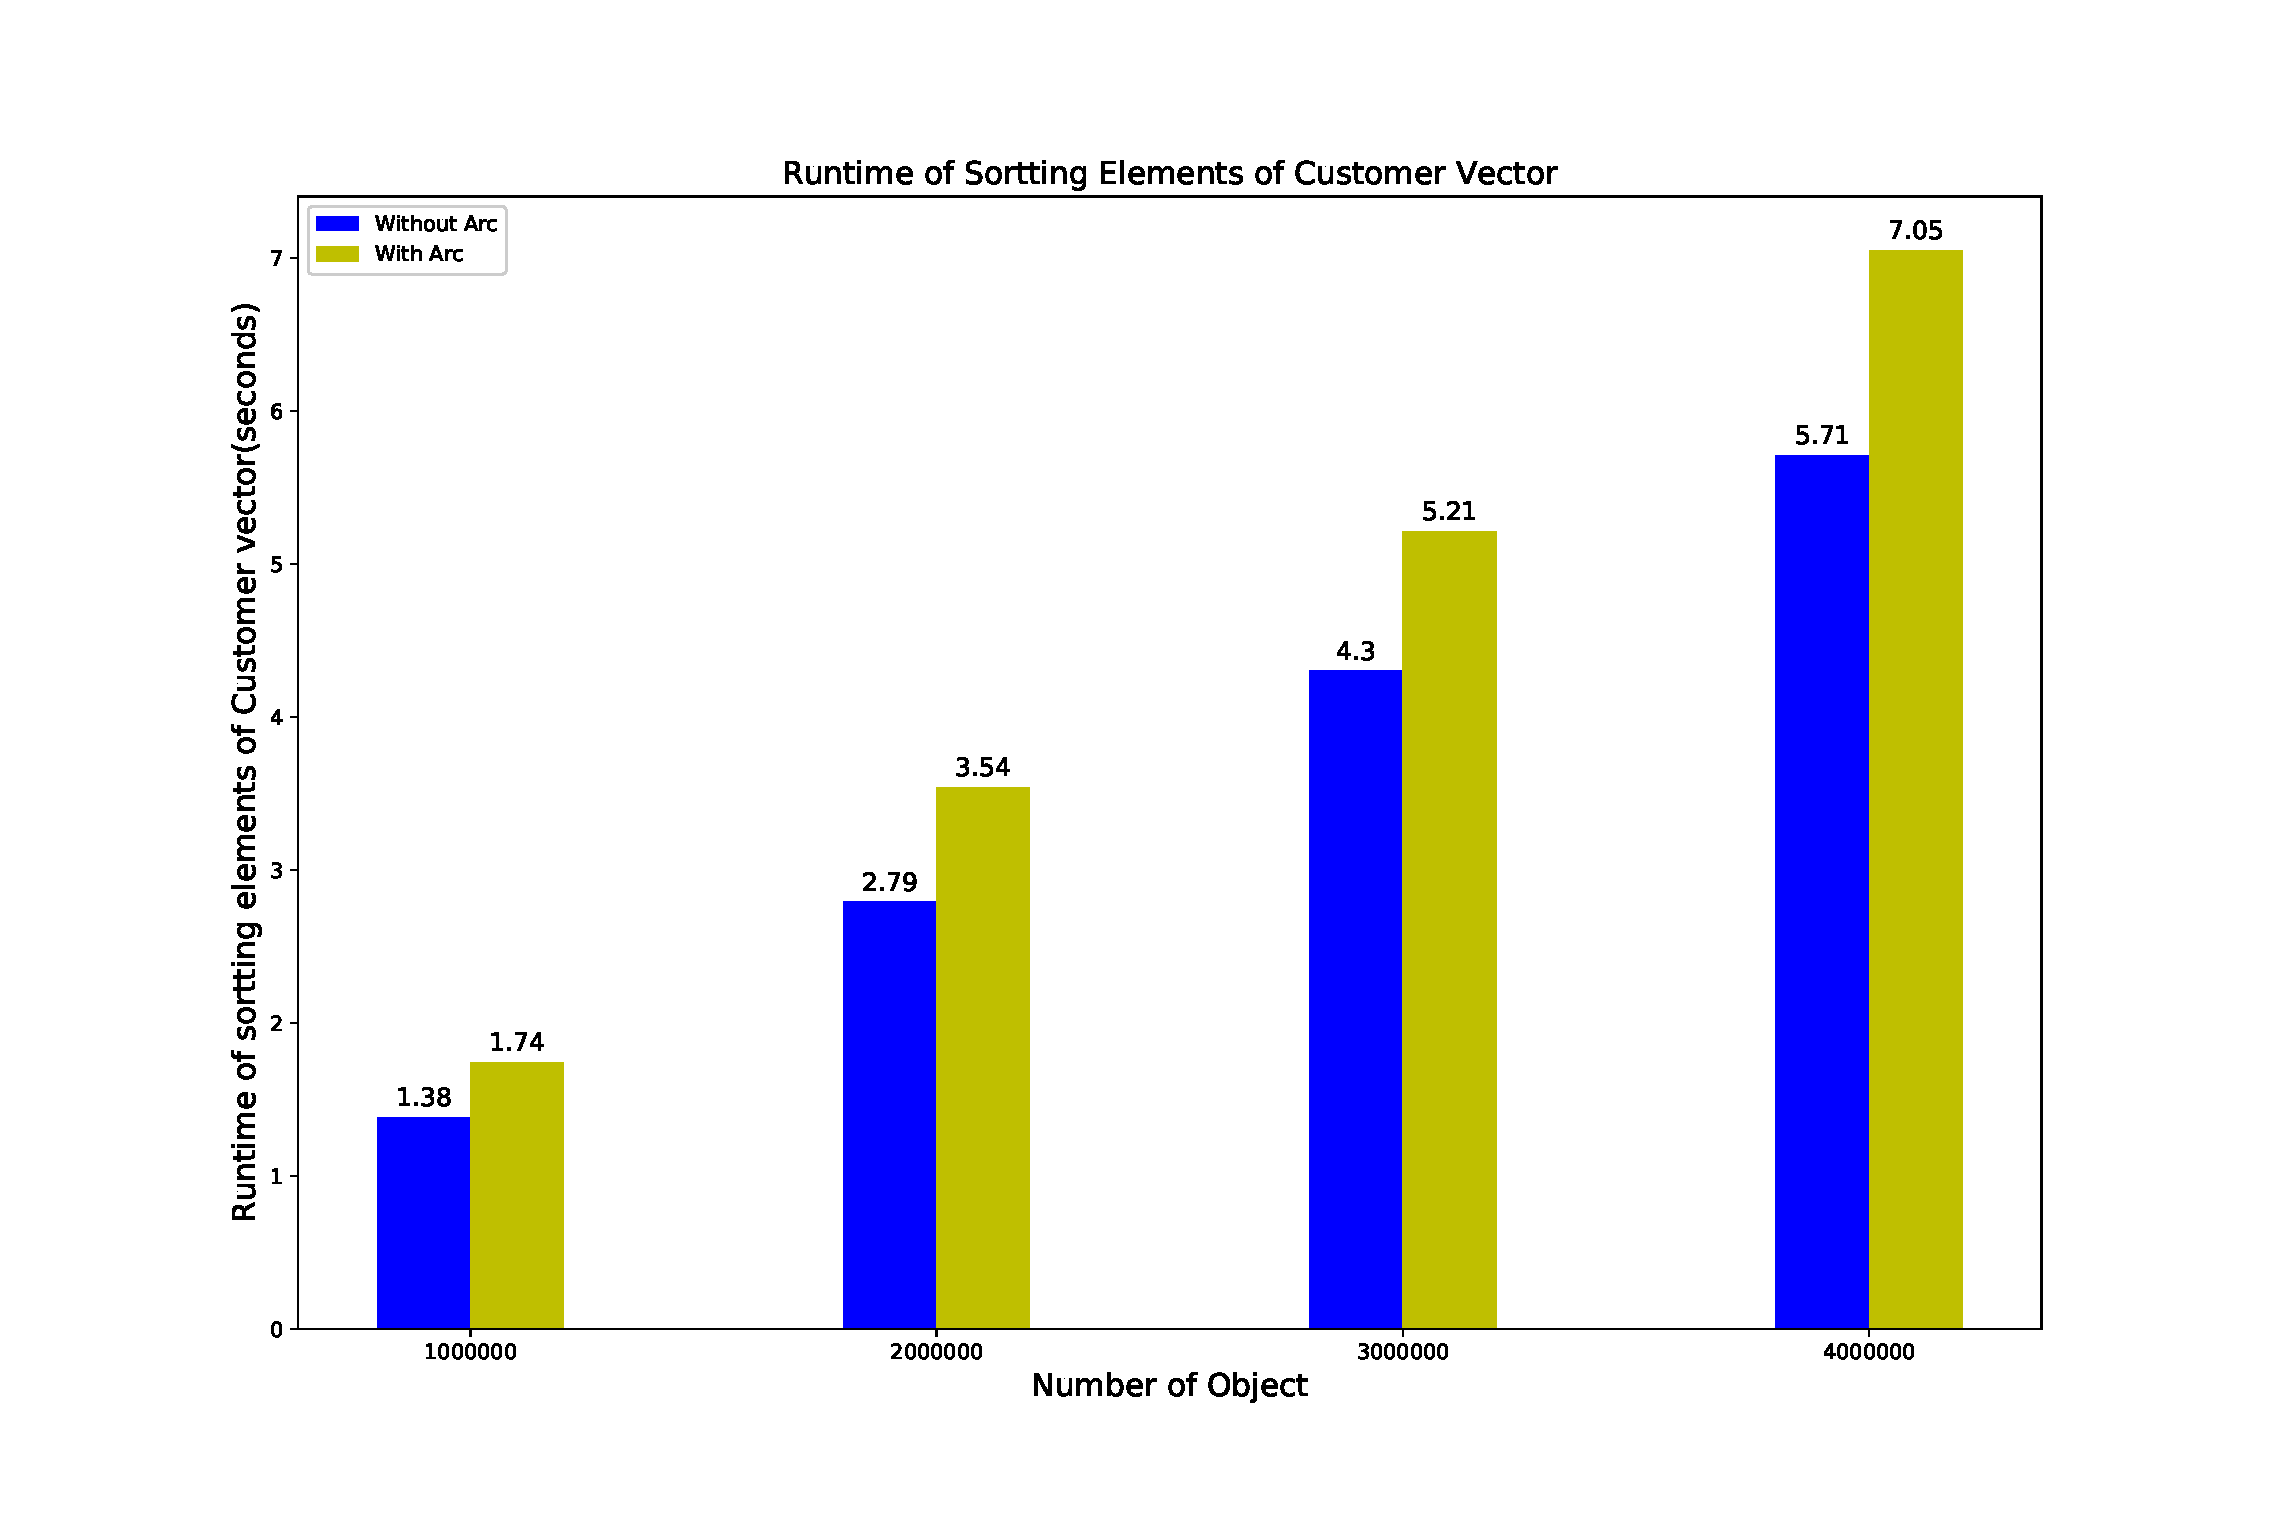
\includegraphics[width=15cm]{rust_merge_sort.eps}
    \caption{Runtime of Sortting Elements of Customer Vector}
    \label{fig:Sampling}
\end{figure}



The other is LinkedList implementation other than vector.
The linkedlist implementation is different from another two. This algorithm is inplace sorting so that it does not de/allocate memory during execution. 
The comparison among vector and linkedlist implementations can show trade-off between contiguous memory access and inplace non memory de/allocation. 
Experiment with Java linkedlist implementation can be interesting, because Java GC is severe problem when number of object is large. 

Of course, there must be a Table of Contents at the beginning of the thesis.